\documentclass[tikz, margin=10mm]{standalone}
\usetikzlibrary{backgrounds}

\begin{document}
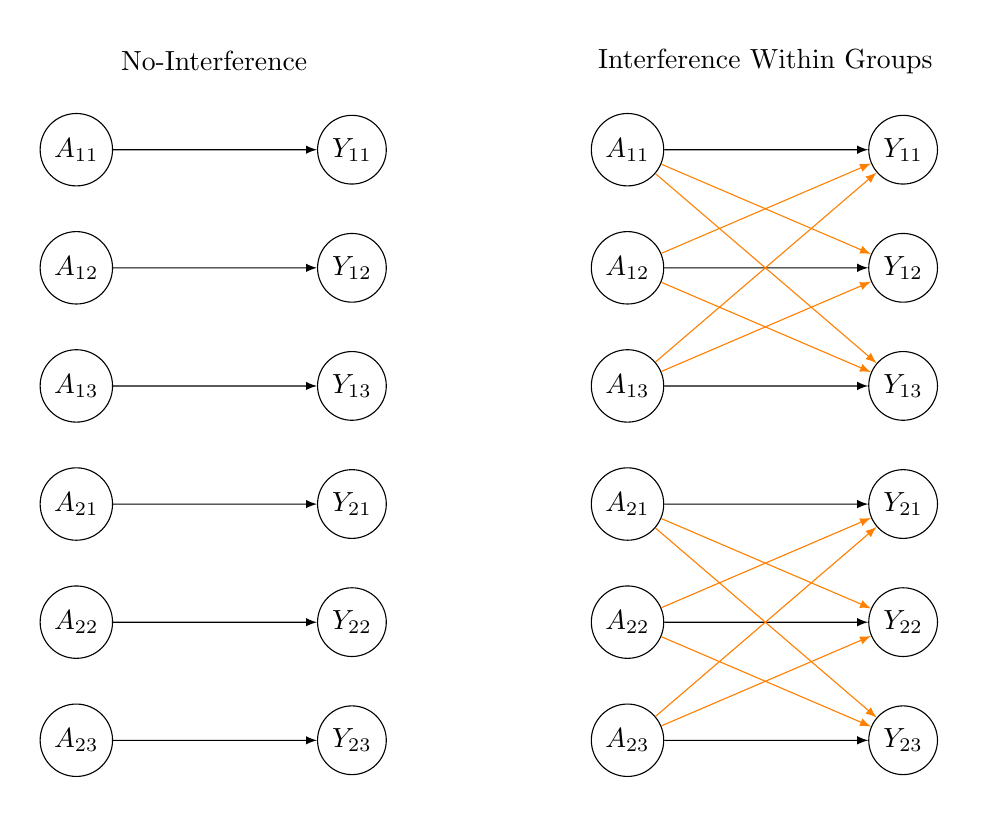
\begin{tikzpicture}[xscale=1.75, yscale=1.5, background rectangle/.style={fill=white}, show background rectangle, ]

\begin{scope}[local bounding box=first figure]

\def\n{6}

\def\Alabels{{"$A_{11}$", "$A_{12}$", "$A_{13}$", "$A_{21}$", "$A_{22}$", "$A_{23}$"}}
\def\Ylabels{{"$Y_{11}$", "$Y_{12}$", "$Y_{13}$", "$Y_{21}$", "$Y_{22}$", "$Y_{23}$"}}

\foreach \i in {1,2,...,\n}
{
  \node (A\i) [circle, draw, inner sep = 3pt] at (0.5, -\i+.5) {\pgfmathparse{\Alabels[\i-1]}\pgfmathresult};
  \node (Y\i) [circle, draw, inner sep = 3pt] at (2.5, -\i+.5) {\pgfmathparse{\Ylabels[\i-1]}\pgfmathresult};
  \draw [-latex] (A\i) -- (Y\i);
}

\node [align=center] at (1.5, 0.25) {No-Interference};

\end{scope}

\begin{scope}[shift={(4,0)}, local bounding box=second figure]

\def\n{6}

\def\Alabels{{"$A_{11}$", "$A_{12}$", "$A_{13}$", "$A_{21}$", "$A_{22}$", "$A_{23}$"}}
\def\Ylabels{{"$Y_{11}$", "$Y_{12}$", "$Y_{13}$", "$Y_{21}$", "$Y_{22}$", "$Y_{23}$"}}

\foreach \i in {1,2,...,\n}
{
  \node (A\i) [circle, draw, inner sep = 3pt] at (0.5, -\i+.5) {\pgfmathparse{\Alabels[\i-1]}\pgfmathresult};
  \node (Y\i) [circle, draw, inner sep = 3pt] at (2.5, -\i+.5) {\pgfmathparse{\Ylabels[\i-1]}\pgfmathresult};
  \draw [-latex] (A\i) -- (Y\i);
}

  \draw [-latex, orange] (A1) -- (Y2);
  \draw [-latex, orange] (A1) -- (Y3);
  \draw [-latex, orange] (A2) -- (Y1);
  \draw [-latex, orange] (A2) -- (Y3);
  \draw [-latex, orange] (A3) -- (Y1);
  \draw [-latex, orange] (A3) -- (Y2);

  \draw [-latex, orange] (A4) -- (Y5);
  \draw [-latex, orange] (A4) -- (Y6);
  \draw [-latex, orange] (A5) -- (Y4);
  \draw [-latex, orange] (A5) -- (Y6);
  \draw [-latex, orange] (A6) -- (Y4);
  \draw [-latex, orange] (A6) -- (Y5);

\node at (1.5, 0.25) {Interference Within Groups};

\end{scope}
\end{tikzpicture}

\end{document}
